\section{Method}


The proposed VideoDescriptor pipeline is designed in such a way to be general to different video understanding tasks, with each of the 4 major steps allowing for multiple methods, or being optional for some tasks.
The VideoDescriptor pipeline is similar to VideoChat-Text of VideoChat \cite{videochat}; the strategy is to represent video as a sequence of textual descriptions, which are then used downstream.
For the purposes of this work, a ``clip" is a small segment of a video that is a few seconds long, 
and is highly cohesive in what it depicts. For example, in a movie, a clip might be a single shot.
At a high level, the pipeline is as follows:
\begin{enumerate}
      \item Partition the video into individual clips.
      \item From each clip, select a small subset of frames to represent the clip.
      \item Using the selected frames, generate a textual description for each clip using an LLM.
      \item Using the textual descriptions, retrieve clips relevant to a question or query.
\end{enumerate}

For brevity, these steps will be referred to as ``Clip partitioning", ``Frame selection", ``Clip description", and ``Clip Retrieval" respectively.
The two most applicable tasks for this pipeline are video retrieval and visual video summarization.
In video retrieval, given a query, the goal is to retrieve the video in a video dataset that best matches the query.
In visual video summarization, the goal is to edit a video down to a shorter length, containing only clips relevant to a given query.

\begin{figure}[h]
      \centering
      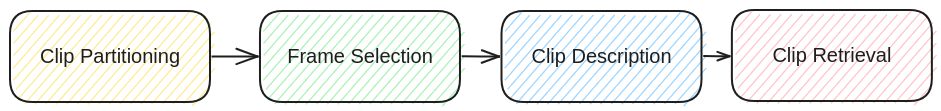
\includegraphics[width=0.8\textwidth]{figures/pipeline.png}
      \caption{High level block diagram of the proposed video understanding pipeline.}
      \label{fig:pipeline}
\end{figure}



\subsection{Clip Partitioning}

Videos can contain a lot of different clips, which may or may not be related.
As such, it's desirable to process and describe each clip individually; clips are an atomic unit of video in this approach.
The input for clip partitioning is the whole video, and the output is a list of breaks (frame numbers) between clips.
The difficult aspect of clip partitioning is to \textit{efficiently} find the boundaries between clips.
A two-hour video at 24 frames per second contains 172,800 frames, and so processing each one is computationally expensive and often infeasible.

The simplest approach to clip partitioning is to simply partition the video into equal-sized clips, without regard for the content of the video.
This approach is simple and fast to compute, but the resulting clips are not necessarily cohesive, since the resulting segments could contain multiple scenes and shots.

\subsubsection{Coarse-to-fine clip partitioning}
A more strategic approach identifies breaks as sequential frames with a large difference between them.
However, even computing a simple difference such as an L1 or L2 norm between each pair of frames is computationally expensive, since a norm must be taken per frame in the video.

As such, the VideoDescriptor pipeline uses a coarse-to-fine approach to clip partitioning.
The algorithm starts by computing the L1 distance between frames \textit{1 second apart}, over the entire video.
If the L1 distance between these frames is above a certain threshold, then its likely that there's a clip break between them.
Thus, the 1-second segment is evaluated frame by frame, and if the distance between two frames is above the threshold, then a clip break is identified.
Empirically, this approach saves 60\% of the L1 computations compared to the naive frame-by-frame approach, and could save more if fewer coarse breaks are identified.

\begin{figure}[h]
      \centering
      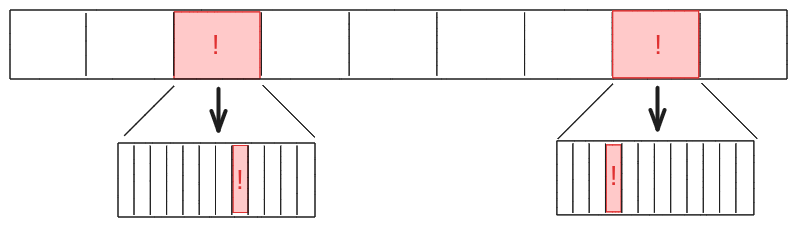
\includegraphics[width=0.6\textwidth]{figures/coarse_to_fine.png}
      \caption{Coarse-to-fine clip partitioning. Vertical lines are frames in the video, and red boxes are identified clip breaks.}
      \label{fig:coarse_to_fine}
\end{figure}


See Figure \ref{fig:breaks} for resulting clip breaks from the coarse-to-fine approach.
Qualitative results show that this approach is very effective at identifying clip breaks, with few false positives and false negatives.

\begin{figure}
      \centering
      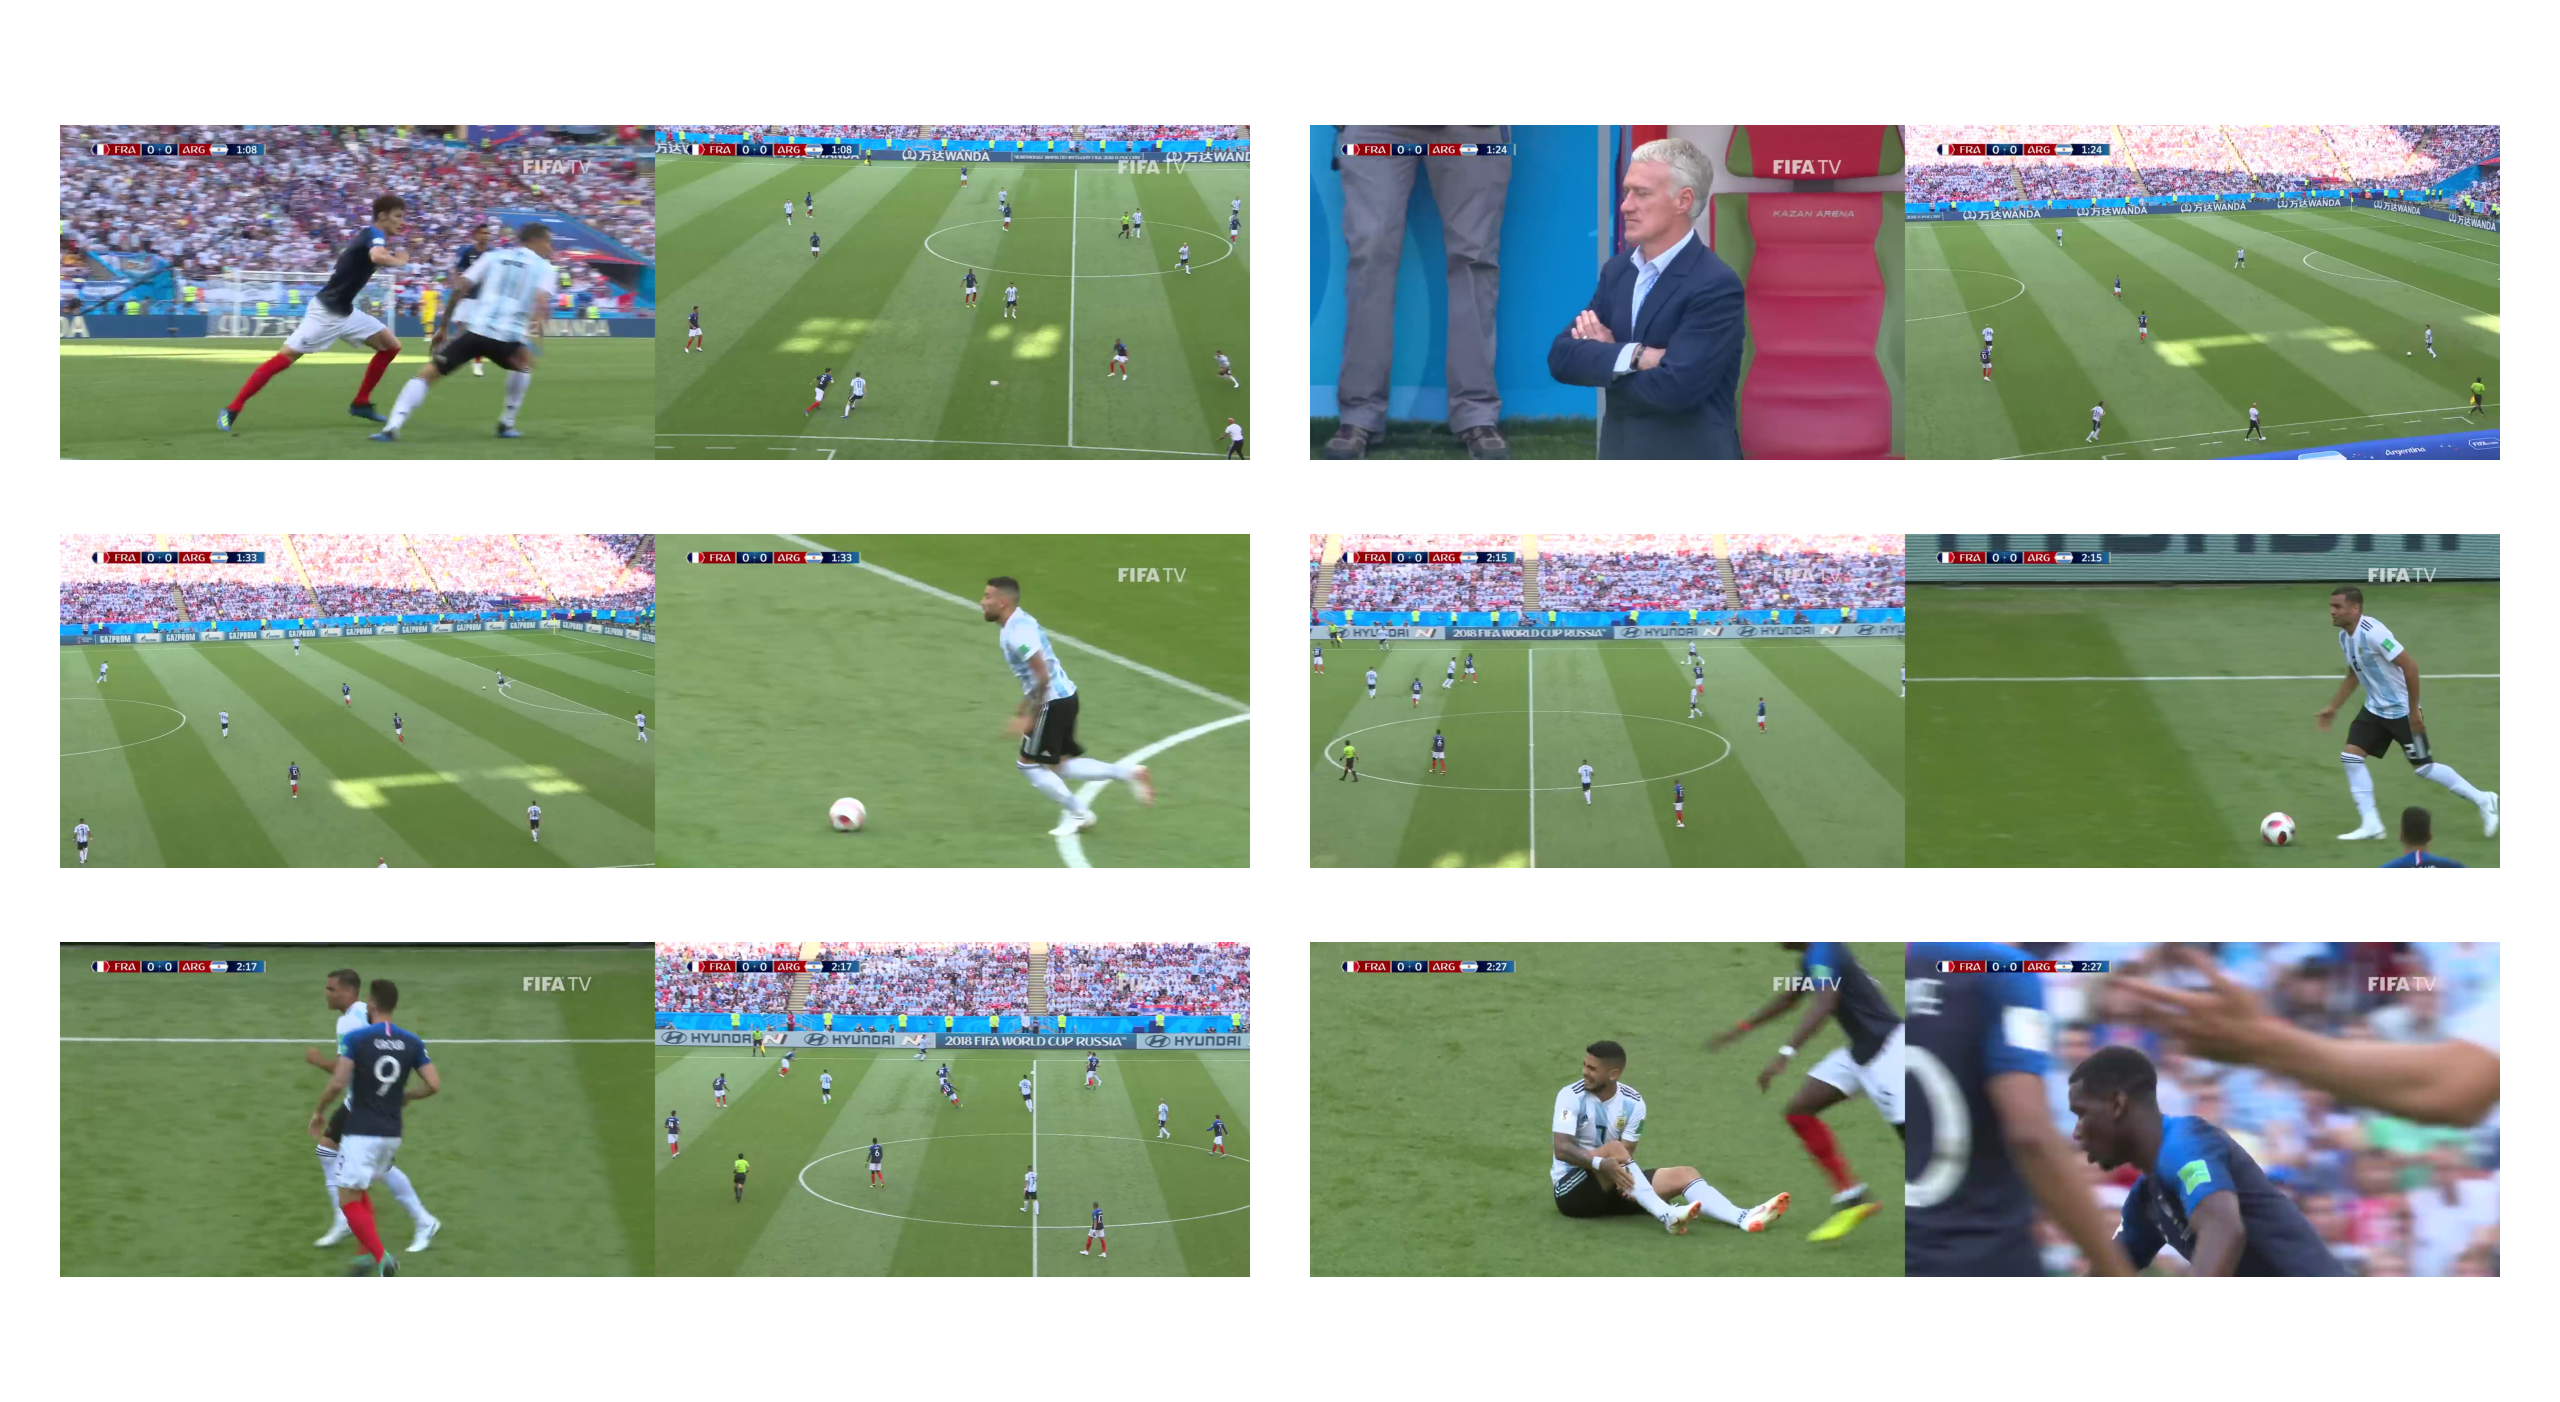
\includegraphics[width=\textwidth]{figures/breaks.png}
      \caption{Frames immediately before and after a clip break, determined by the coarse-to-fine clip partitioning strategy.}
      \label{fig:breaks}
\end{figure}


\subsection{Frame Selection}

Even within a single clip, there are a lot of frames, most of which are very similar to their neighbours.
To make the pipeline efficient, it's critical to select a subset of the most semantically relevant frames.
The input to frame selection is a clip (small segment of video) and the output is a list of frames selected for further processing.
Earlier works simply sample randomly \cite{clipbert} or sample uniformly, at a coarse frame rate such as 1 frame per second \cite{clip4clip}.
This work explores 4 different frame selection strategies:
stratified selection, random sampling, greedy L1 selection, and stratified triplet selection.

\subsubsection{Stratified Selection}
To get a diverse set of frames, the first, last and middle frames of a clip are selected for stratified selection.
For brevity, this sampling method is referred to as \verb|3strat|. 
\verb|5strat| is also explored, which selects the first frame, last frame, and 3 evenly spaced frames in between.

\subsubsection{Random Sampling}
A random sampling approach is also explored, with either 3 or 5 frames selected from the clip (with replacement).
These are referred to as \verb|3rand| and \verb|5rand| respectively.

\subsubsection{Greedy L1 Selection}
The idea for greedy selection is to skip frames that are visually similar to the previously selected frame.
Greedy L1 selection initially selects the first frame of a clip. 
Then, it selects an additional frame if the L1 distance between the new frame and the previously selected frame is greater than some threshold.
The L1 distance is normalized by the number of pixels in the image, so that the threshold is independent of the video resolution.
More formally, the current frame $I_{c}$ is selected if:
\begin{equation}
      c < \frac{|I_{p} - I_{c}|}{W \times H \times C}
\end{equation}

where $c$ is a pre-defined threshold, $|\cdot|$ is L1 distance, $I_{p}$ is the previously selected frame, and $W$, $H$, $C$ are the width, height, and channels of the frames, respectively.
In the MSR-VTT dataset, most videos are quite short (see Figure \ref{fig:length_histogram}), and often only contain a single static shot.
As such, when using greedy L1 selection, a substantial number of videos only have the first frame selected (with L1 threshold 180).
L1 distance was chosen over L2 because L2 is very sensitive to large changes in a few pixels; L1 gives a better sense of the overall change in the image.

\begin{figure}
      \centering
      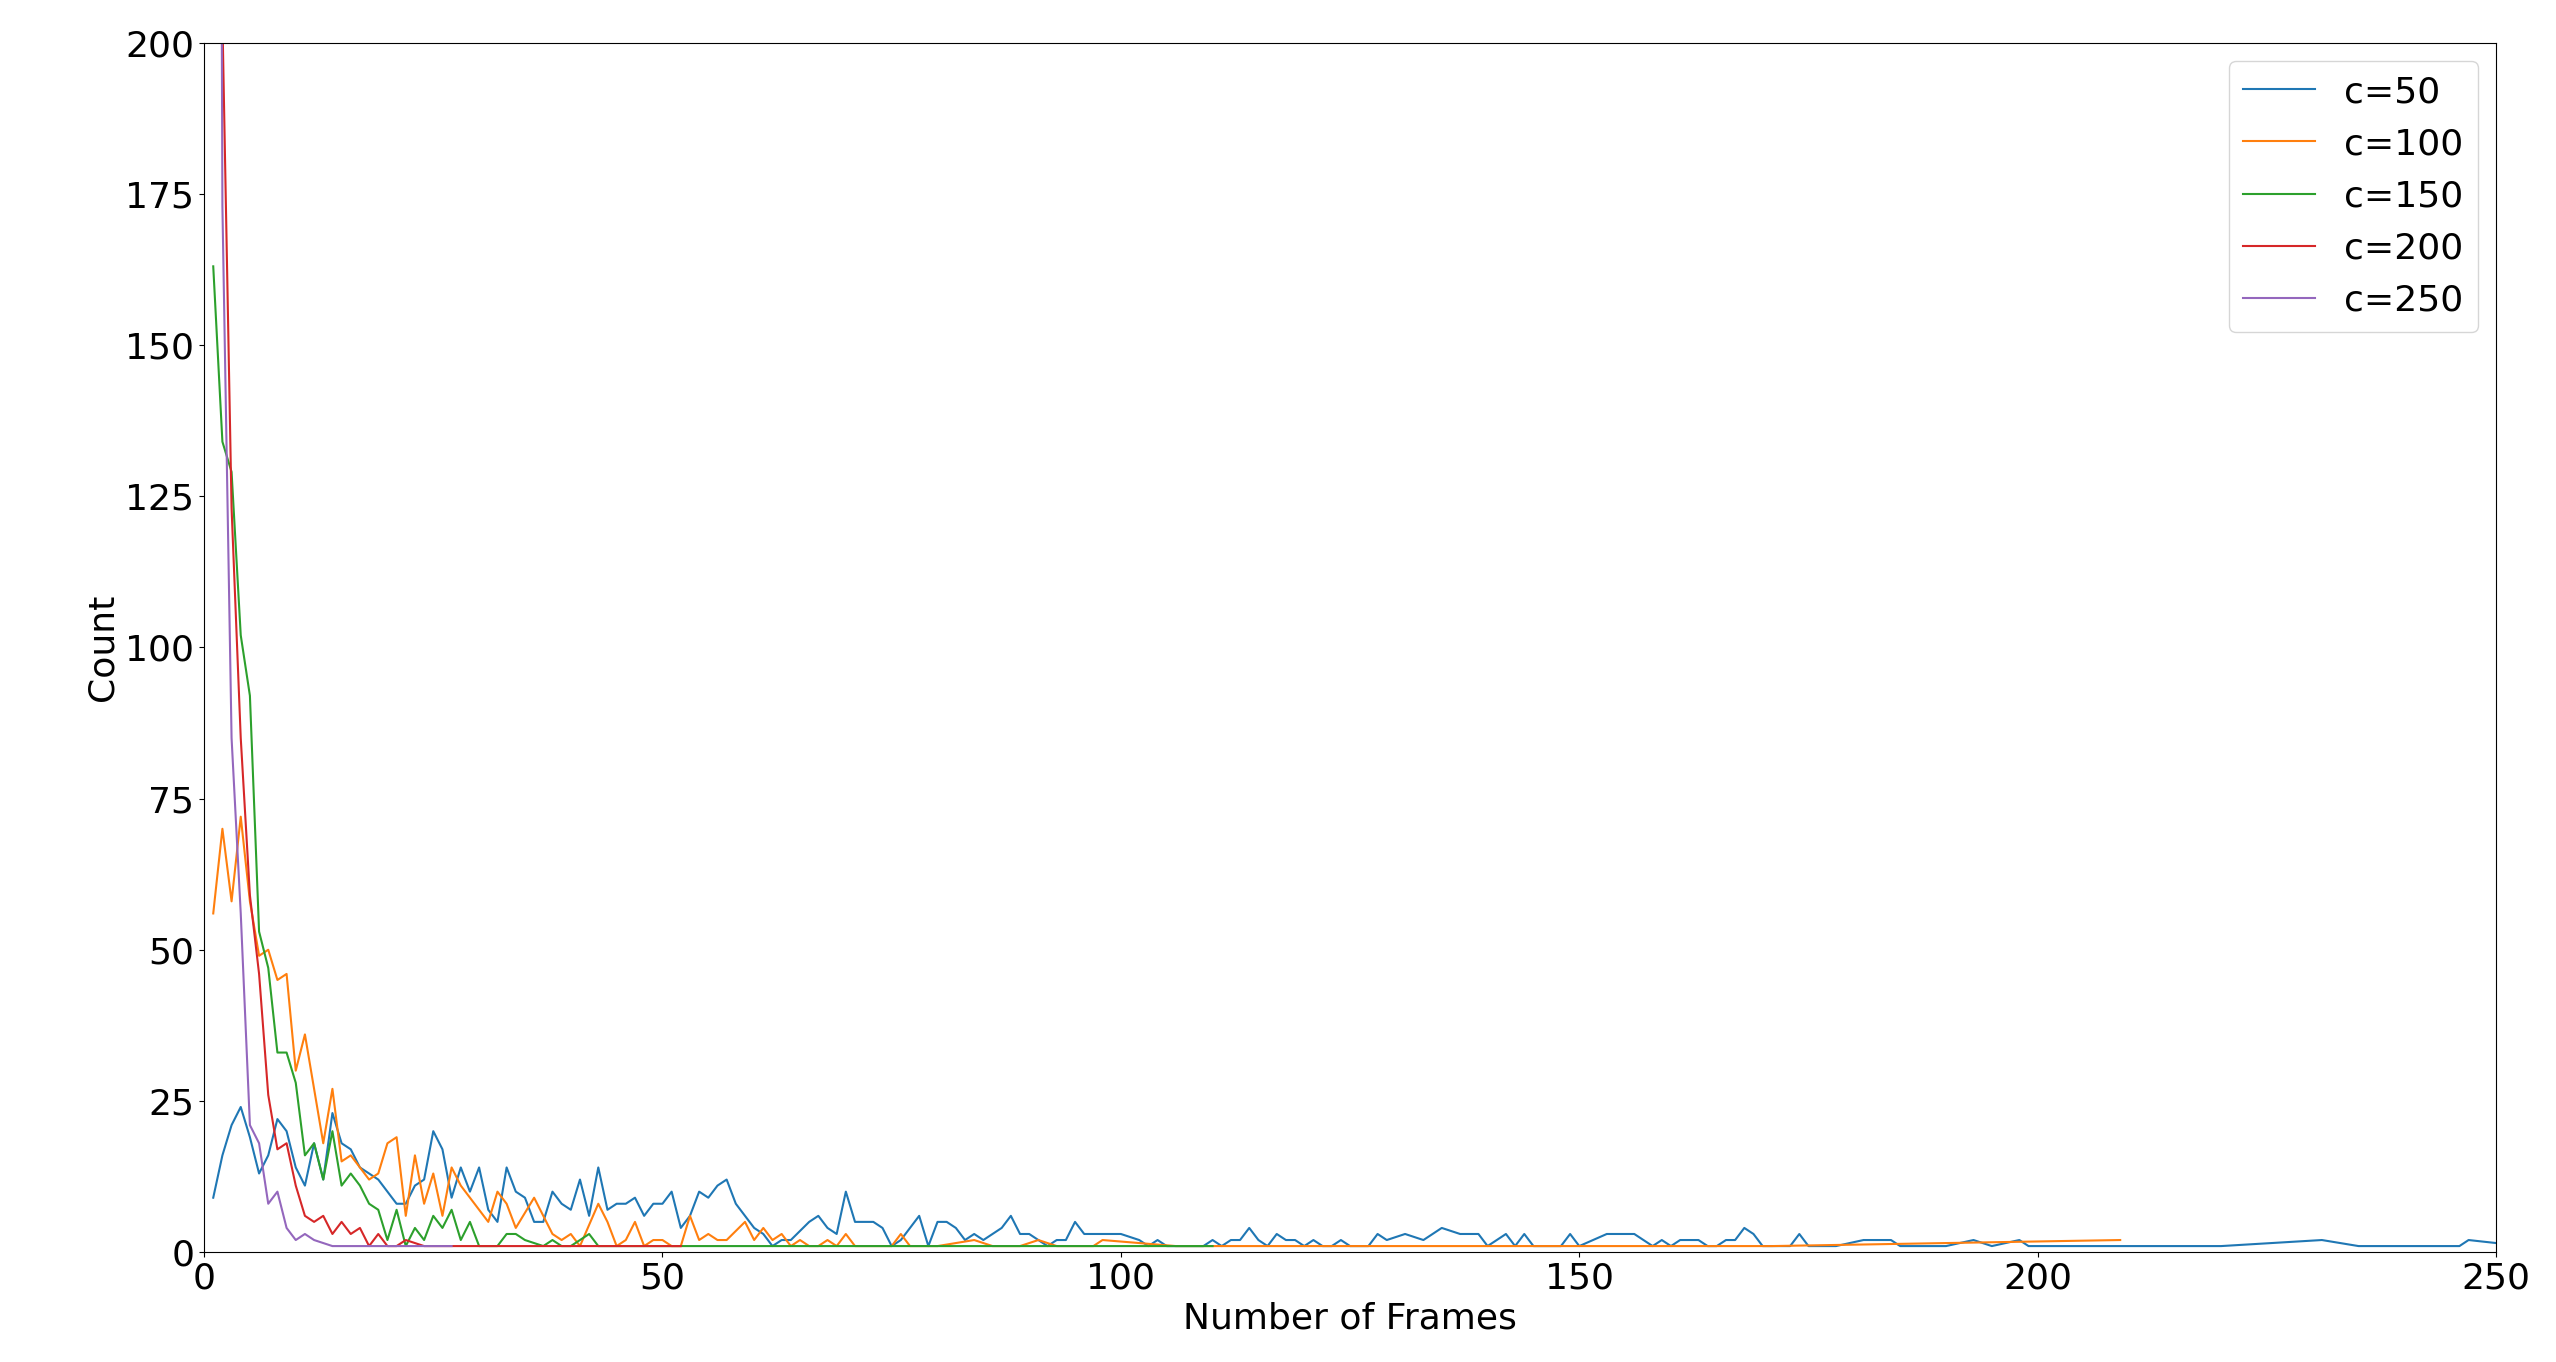
\includegraphics[width=0.8\textwidth]{figures/num_frames_histogram.png}
      \caption{Number of frames selected per video in the MSR-VTT dataset retrieval split when using greedy L1 selection, for different thresholds.}
      \label{fig:optical_flow}
\end{figure}



\subsubsection{Stratified Triplet Selection}
It's possible that single frames at multiple points in the clip are not enough to capture a clip's dynamic content.
For this reason, this work also explores stratified triplet selection, where at each stratified point in the clip, 3 frames are selected across 1 second.
The motivation for this method is that the 3 frames in a single second will show what is changing in the scene, capturing the action in that second.
Each triplet is fed in as a single input into the LLM during clip description.
As a result, there is only one textual description per triplet when using this selection method.

\subsection{Clip Description}

The input to clip description is a prompt and multiple frames, and the output is a text description.
The LLM used in testing this pipeline is LLava \cite{llava}.
LLaVA is selected because it is free and open source, and can be run on a single consumer GPU, making it amenable to experimentation.
While LLaVA can take multiple images as input, it is rarely tested and on multi-image inputs.
So, apart from the stratified triplet selection experiments, most clip descriptions are the concatenation of the descriptions of individual frames.

Two prompts are tried in this work, one of which is is dubbed ``concise" (C), while the other is ``verbose" (V).
The concise prompt is ``Please describe the objects in this image."
The verbose prompt is ``Please describe the objects in this image. Be as descriptive as possible."
The third option used for clip description is dubbed ``temperature" (T), which uses the verbose prompt with a sampling temperature of 0.2. 
Two different responses are generated (using beam search) for each frame and concatenated when using the ``temperature" option.
In all cases, the caption for each frame (or triplet) is limited to 512 words, to bound the amount of computation required per frame.

\subsection{Clip Retrieval}

The last aspect of of the pipeline is, of course, retrieval.
The input to clip retrieval is a query, and the output is a list of clips sorted by relevance.
Because LLMs have described the content of the videos at this point in the pipeline, the retrieval task is reduced to that of text retrieval, which is well-studied.
In this work, we explore two retrieval strategies: BM25 and Bi-Encoder, using OpenAI embeddings.
BM25 is a highly performant sparse retriever, relying on term frequencies and other statistics to rank documents \cite{bm25}. %TODO make sure this citation gets rendered
It is a very fast baseline, retrieving from a thousand documents in milliseconds.

\subsubsection{Bi-Encoder Retrieval}
The Bi-Encoder approach is heavily inspired by DPR \cite{dpr}, but uses the same encoder for both documents and queries, and uses L2 distance as a similarity metric instead of the dot product.
At a high level, all the documents are encoded into a vector space using an LLM encoder, and the query is encoded into the same vector space using the same encoder.
Then, the similarity between the query and each document is computed using L2 distance, and the top-k documents are returned in a retrieval.
While different in application, it's very similar to the bi-encoder strategy used in the BLINK zero-shot entity linker \cite{blink}.
See Figure \ref{fig:bienc} for a visual representation of the bi-encoder retrieval strategy.
The encoder used to generate embedding vectors is the OpenAI model \verb|text-embedding-ada-002|, which outputs 1536-dimensional vectors.
The KNN is performed using the FAISS library \cite{faiss}, and all clip descriptions are embedded and stored in an index beforehand, making querying for nearest neighbours very fast.

\begin{figure}
      \centering
      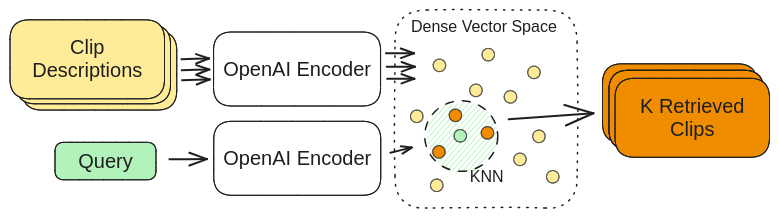
\includegraphics[width=0.8\textwidth]{figures/openai_DPR.png}
      \caption{Bi-Encoder retrieval strategy, using OpenAI embedding API.}
      \label{fig:bienc}
\end{figure}

